% !TEX program = xelatex
% !BIB program = bibtex

\documentclass[UTF8,cs4size]{ctexart}

% layout
\usepackage[left=3cm,right=3cm]{geometry}
\linespread{1.25}
\ctexset{
  section = {
    name = \S
  },
  subsection/name = \S,
  subsubsection/name = \S
}
% \makeatletter
% \def\@seccntformat#1{%
%   \expandafter\ifx\csname c@#1\endcsname\c@section
%   Section \thesection:
%   \else
%   \csname the#1\endcsname\quad
%   \fi}
% \makeatother
 
% page headings
\usepackage{fancyhdr}
\setlength{\headheight}{15.2pt}
\pagestyle{fancy}
\lhead{\leftmark}
\rhead{M201873026 刘一龙}
\cfoot{\thepage}
% \makeatletter
% \let\headauthor\@author
% \makeatother

% footnote
\renewcommand\thefootnote{\fnsymbol{footnote}}

% url/ref
\usepackage{hyperref}
\hypersetup{
  colorlinks,
  citecolor=black,
  filecolor=black,
  linkcolor=black,
  urlcolor=black,
  pdfauthor={刘一龙},
  pdftitle={人工智能课程设计报告}
}

% vertical centering title page
\usepackage{titling}
% \renewcommand\maketitlehooka{\null\mbox{}\vfill}
\renewcommand\maketitlehookd{\vfill\null}

% table of contents
\usepackage{tocloft}
\renewcommand\cftsecfont{\normalfont}
\renewcommand\cftsecpagefont{\normalfont}
\renewcommand{\cftsecleader}{\cftdotfill{\cftsecdotsep}}
\renewcommand\cftsecdotsep{\cftdot}
\renewcommand\cftsubsecdotsep{\cftdot}
\renewcommand\cftsubsubsecdotsep{\cftdot}
\renewcommand{\contentsname}{\hfill\bfseries\Large 目录\hfill}   
\setlength{\cftbeforesecskip}{10pt}

% figures
\usepackage{graphicx}
\graphicspath{figures/}
% \newcommand\figureht{\dimexpr
%   \textheight-3\baselineskip-\parskip-.2em-
%   \abovecaptionskip-\belowcaptionskip\relax}

% tables
\usepackage{caption} 
\captionsetup[table]{skip=10pt}

% math, algorithms, code
\usepackage{amsmath,amssymb,url}
\usepackage{algorithm,algorithmicx,algpseudocode}
\usepackage{listings}

\lstset{
   extendedchars=true,
   basicstyle=\footnotesize\ttfamily,
   showstringspaces=false,
   showspaces=false,
   numbers=left,
   numberstyle=\footnotesize,
   numbersep=9pt,
   tabsize=2,
   breaklines=true,
   showtabs=false,
   captionpos=b
}

% bibliography
\usepackage[super,square,comma,sort]{natbib} % for \citet and \citep
\renewcommand{\refname}{\S 参考文献}
% \begin{filecontents}{report.bib}
% \end{filecontents} 

% appendix
\usepackage{appendix}

\title{{\LARGE《\textbf{人工智能}》课程设计报告}\\ \bigskip \bigskip \bigskip {\Large 选题名称:\textbf{GBA - 一个基于蒙特卡洛树搜索的简单五子棋人工智能系统}} \vspace{7cm}}
\author{计算机科学与技术学院\\ 硕1801班\\ \textbf{M201873026}\\ \textbf{刘一龙}}
\date{2018年11月}

\begin{document}

\pagenumbering{gobble} % no page number
\maketitle
\newpage
\null\thispagestyle{empty}
\newpage

\pagenumbering{roman}
\section*{\S 摘要}\sectionmark{\S 摘要}
\addcontentsline{toc}{section}{\S 摘要}
本文提出实现 GBA(GoBang Ai)系统,一个基于蒙特卡洛树搜索的简单五子棋人工智能系统,
将最简单的基于 UCT 的蒙特卡洛树搜索策略移植到五子棋游戏上。
本文首先介绍了蒙特卡洛搜索树算法,然后阐述了 GBA 系统的整体实现,最后阐述了该系统中关于对弈算法的关键优化。
该系统能够进行稳定的对弈,能够对于简单的活四/成五的局势进行阻断,并展开一定强度的进攻。
\newpage

\pagenumbering{gobble} % no page number

\null\thispagestyle{empty}
\newpage
\tableofcontents
\newpage
\null\thispagestyle{empty}
\newpage

\pagenumbering{arabic}

\section{引言}
游戏 AI 的经典方法要求很高领域知识的质量,或长时间生成有效的AI行为。
这两个特点妨碍建立具有挑战性的游戏AI的目标。
在实现游戏 AI 时,最重要的是评估游戏状态或游戏局势的函数。
经典的方法是使用启发式方法,利用领域知识建立这样的估计函数。
但是,基于启发式方法建立估计函数是一个复杂的任务。
它是复杂游戏环境中游戏 AI 较弱的一个重要原因。

由于 Google DeepMind 的 AlphaGo\cite{DBLP:journals/nature/SilverHMGSDSAPL16}与 AlphaGo Zero\cite{silver2017mastering}的横空出世,
使得人们将目光聚焦至蒙特卡洛树搜索(MCTS,Monte-Carlo Tree Search)\cite{wiki:Monte_Carlo_tree_search}这一上世纪就出现的数学方法。
其又被称为随机抽样或统计试验方法,属于计算数学的一个分支。蒙特卡洛模拟\cite{binder1993monte}最早用于统计物理领域。

其实在很早以前,便有学者提出蒙特卡洛树搜索可以有效地应用于棋盘游戏\cite{DBLP:conf/aiide/ChaslotBSS08}。
蒙特卡罗树搜索作为游戏 AI 的新颖统一框架,通过游戏状态空间的随机探索用来预测最有希望的游戏动作。
最早在 1993 年\cite{brugmann1993monte},就有学者将蒙特卡洛模拟运用在 9x9 的围棋游戏中。
后来有学者将蒙特卡洛树搜索与 UCB(Upper Confidence Bound)相结合提出了 UCT(Upper Confidence Bound Apply to Tree)算法\cite{DBLP:conf/ecml/KocsisS06}。
MoGo 程序\cite{DBLP:conf/cig/WangG07}\cite{DBLP:conf/icml/GellyS07}利用 UCT 算法将自身胜率提升了将近一倍,并成功击败了棋力强劲的围棋业余选手。
10 年后的今天,DeepMind 的学者研制出的 AlphaGo 人工智能更是成功地击败了人类顶尖围棋选手柯洁。

本文提出实现 GBA(GoBang Ai)系统\footnote{本系统的在线版已发布于~\href{http://ai.hust.cf}{ai.hust.cf},
可以访问该网站与 GBA 系统进行对弈。},一个基于蒙特卡洛树搜索的简单五子棋人工智能系统,将最简单的基于 UCT 的蒙特卡洛树搜索策略移植到五子棋游戏上。
本文首先介绍蒙特卡洛搜索树算法,然后阐述 GBA 系统的整体实现,最后阐述该系统中关于对弈算法的关键优化。
\newpage

\section{蒙特卡洛树搜索}
蒙特卡罗树搜索(MCTS),是一种使用随机模拟的最佳优先原则的搜索算法。其基本过程如图~\ref{fig:mcts_phase}所示。
在阶段(1)中,现有信息用于重复选择连续的子节点直到搜索树的末尾。接下来,在阶段(2)中,通过添加节点来扩展搜索树。
然后,在阶段(3)中,模拟运行到最后以确定获胜者。
最后,在阶段(4)中,使用从模拟游戏获得的新信息更新所选路径中的所有节点。
重复运行这种 4 阶段算法,直到收集到足够的信息以产生良好的下一步选择。
重要的是要注意搜索树在结构上与游戏树相同,并且搜索树还包含从模拟中收集的统计信息,搜索树是整个游戏树的一个子集。

\begin{figure}[htb]
  \centering
  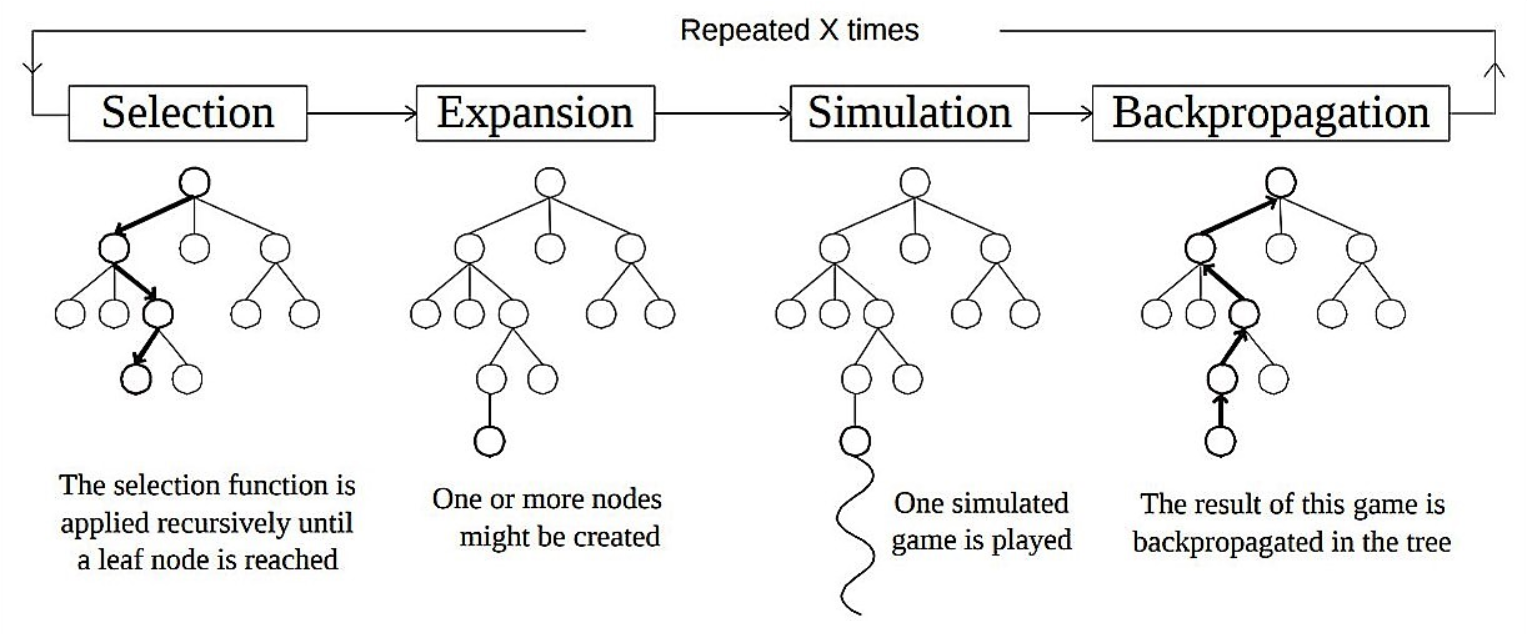
\includegraphics[width=\textwidth,height=5cm]{figures/final_mcts_phase.png}
  \caption{MCTS 算法基本过程\cite{DBLP:conf/aiide/ChaslotBSS08}}
  \label{fig:mcts_phase}
\end{figure}

\subsection{结点选择(Selection)}
从搜索树的根节点开始,通过重复(1)选择合法移动和(2)前进到相应的子节点来扩展树。
如果节点中的一个,几个或所有合法移动在搜索树中没有相应的节点,便会停止选择。
在树中找到状态时,根据存储的统计数据选择下一个操作,以便在开发和探索(Exploration Term and Exploitation Term)之间取得平衡。
一方面,任务通常是选择导致迄今为止最佳结果的游戏动作(利用);另一方面,由于评估(探索)的不确定性,仍然需要探索不太有希望的行动,
即应该探索获取信息的新途径,同时利用现有信息来利用已知良好的路径。

一种(坏)方法是随机选择路径。 随机选择可以很好地探索,但它根本没有利用已知信息。
另一种(同样糟糕的)方法是使用每个节点的平均赢率,这实现了很好地利用了已知信息,但在无法探索更多未知路径。
有学者提出利用 UCB(Upper Confidence Bound)公式来决定下一节点的选择\cite{DBLP:conf/ecml/KocsisS06},
当将其应用于蒙特卡洛树搜索时,被称为 UCT(Upper Confidence Bound Apply to Tree)算法。

\begin{equation}
  \text{UCT} = \frac{w_i}{s_i} + c\sqrt{\frac{\ln{s_p}}{s_i}}
  \label{eq:uct}
\end{equation}

公式~\eqref{eq:uct}称为“UCT 函数”,分为 2 部分:左部为利用值,右部为探索值。其中,
$w_i$ 表示此节点的模拟次数导致获胜;
$s_i$ 表示此节点的模拟总数;
$s_p$ 表示父节点的模拟总数;
$c$ 表示探索参数。
$\frac{w_i}{s_i}$ 表示当前节点的游戏平均胜率,当选择该值较大的节点时,可以很好地利用已知信息做出下一步行动;
$\sqrt{\frac{\ln{s_p}}{s_i}}$ 表示当前节点的模拟频率(被遍历的概率),当选择该值较大的节点(较少模拟)时,可以很好地探索未知路径。
探索参数 $c$ 只是可以选择的一个数字,它控制着等式中利用值与探索值之间的权重大小,选择的通常数字是 $c = \sqrt{2}$。

每次需要在多个子节点之间进行选择时,便使用公式~\eqref{eq:uct}(即 UCT 函数)来获取每个子节点的 UCT 值,并选择具有最大值的子节点。
在选择阶段,使用 UCT 选择功能来决定选择哪个子节点。
反之,UCT 函数使用子节点的获胜次数 $w_i$ 和模拟次数 $s_i$ 以及父节点的模拟次数 $s_p$ 来生成每个子节点的 UCT 值。
此信息在反向传播阶段(即第 4 阶段)更新,因此,获得此迭代的信息将影响下一次迭代的移动选择,依此类推。

\subsection{结点扩展(Expansion)}
选择阶段结束后,搜索树中将至少有一个未访问的移动(以下称为未扩展移动,Unexpanded Play)。
随机选择一个未展开的移动,然后创建与该移动相对应的子节点(如图~\ref{fig:mcts_phase}所示)。
将此节点作为子节点添加到选择阶段中的最后一个选定节点,从而扩展搜索树。
节点中的统计信息初始化为 0 次模拟与 0 次胜利(即 $w_i = 0$,$s_i = 0$)。

\subsection{搜索树模拟(Simulation)}
对于游戏的其余部分,随机选择动作直到游戏结束(决出胜者或达成和局),这一过程称为搜索树模拟。
从扩展阶段中新创建的节点继续,随机选择移动并重复进行游戏状态。
在这个阶段,只是简单地应用游戏规则来重复(1)找到当前游戏状态下的所有合法移动,(2)随机选择一个合法移动,然后(3)推进游戏状态。
不存储此过程的任何部分,当到达游戏结束的状态时,此阶段结束。
即这一过程重复进行,直到比赛结束,都不会创建新节点。
动作选择概率的适当加权对游戏水平具有显着影响。
如果以相同的概率选择所有行动,则所采用的策略通常较弱,并且蒙特卡洛搜索的水平不是最理想的。

\subsection{状态回播(Backpropagation)}
在一轮模拟阶段结束之后,更新所有访问节点(即从根节点开始至结束节点路径上的所有节点)的统计数据(如图~\ref{fig:mcts_phase}所示),这一过程称为状态回播。
每个被访问节点的模拟计数 $s_i$ 递增。
根据哪个玩家获胜,其获胜次数 $w_i$ 也可以递增。
若黑方获胜,因此每个访问的白色节点的获胜计数都会增加。
这是由于每个节点的统计数据用于其父节点的选择,而不是它自己的选择。

\subsection{选择最优行动}
重复上述 4 个步骤,进行完足够的迭代后,搜索树上会存储足够的游戏信息,
用于选出下一步理想中最优的行动。
例如,可以简单地选取 $\frac{w_i}{s_i}$ 最大值的子节点作为下一步行动。

\clearpage

\section{五子棋系统概述}
\subsection{五子棋游戏框架实现}
本游戏利用 React\cite{web:react}框架实现,将图形界面封装为三个组件,并将逻辑模块绑定至相关点击事件。
\subsubsection{游戏主流程}
在玩家点击棋盘一个完成落子后,GBA 系统会根据棋局当前局势,利用蒙特卡洛树搜索,在给定的时限内(不同的时限会影响 GBA 系统的强度)给出落子选择。
GBA 系统落子完毕后,玩家可以继续落子,直到决出胜者或达成和局,如流程~\ref{alg:game_main}所示。

\begin{algorithm}
  \floatname{algorithm}{流程}
	\algrenewcommand\algorithmicrequire{\textbf{输入:}}
	\algrenewcommand\algorithmicensure{\textbf{输出:}}
	\caption{游戏主流程}
	\label{alg:game_main}
  \begin{algorithmic}[1]
    \While{未决出胜者 $OR$ 未达成和局}
      \State handleClick($row$, $col$)
      \State $play \gets$ ($row$, $col$)
      \State $newState \gets$ StateMachine.nextState($state$, $play$)
      \State $aiPlay \gets$ AI.bestPlay($newState$)
      \State $newState \gets$ StateMachine.nextState($newState$, $aiPlay$)
    \EndWhile
    \State \textbf{return} $newState$
	\end{algorithmic}  
\end{algorithm}

\subsubsection{游戏核心模块}
\paragraph{StateMachine.js}
实现了一些与游戏状态相关的函数,如 nextState、isDeadGame、checkWinner 等。
\paragraph{MCTS.js}
实现了蒙特卡洛树搜索策略,对外提供了 2 个 API:MCTS.runSearch 与 MCTS.bestPlay。
\paragraph{AI.js}
实现了 GBA 系统,利用 MCTS.js 提供的 API 构建完整的五子棋人工智能。
\paragraph{Game.js}
实现了五子棋游戏的主要逻辑,如 mainLoop、load/storeState、changeGameMode 等。
图形界面的各种点击事件主要是由 Game.js 模块的各个函数进行处理的。
\subsubsection{界面设计}
利用 React 框架,遵循组件复用原则,利用 Cell 与 Grid 组件构建了 Gobang,
最后完成了五子棋游戏的图像界面。游戏界面如图~\ref{fig:UI}所示。

\begin{figure}[htb]
  \centering
  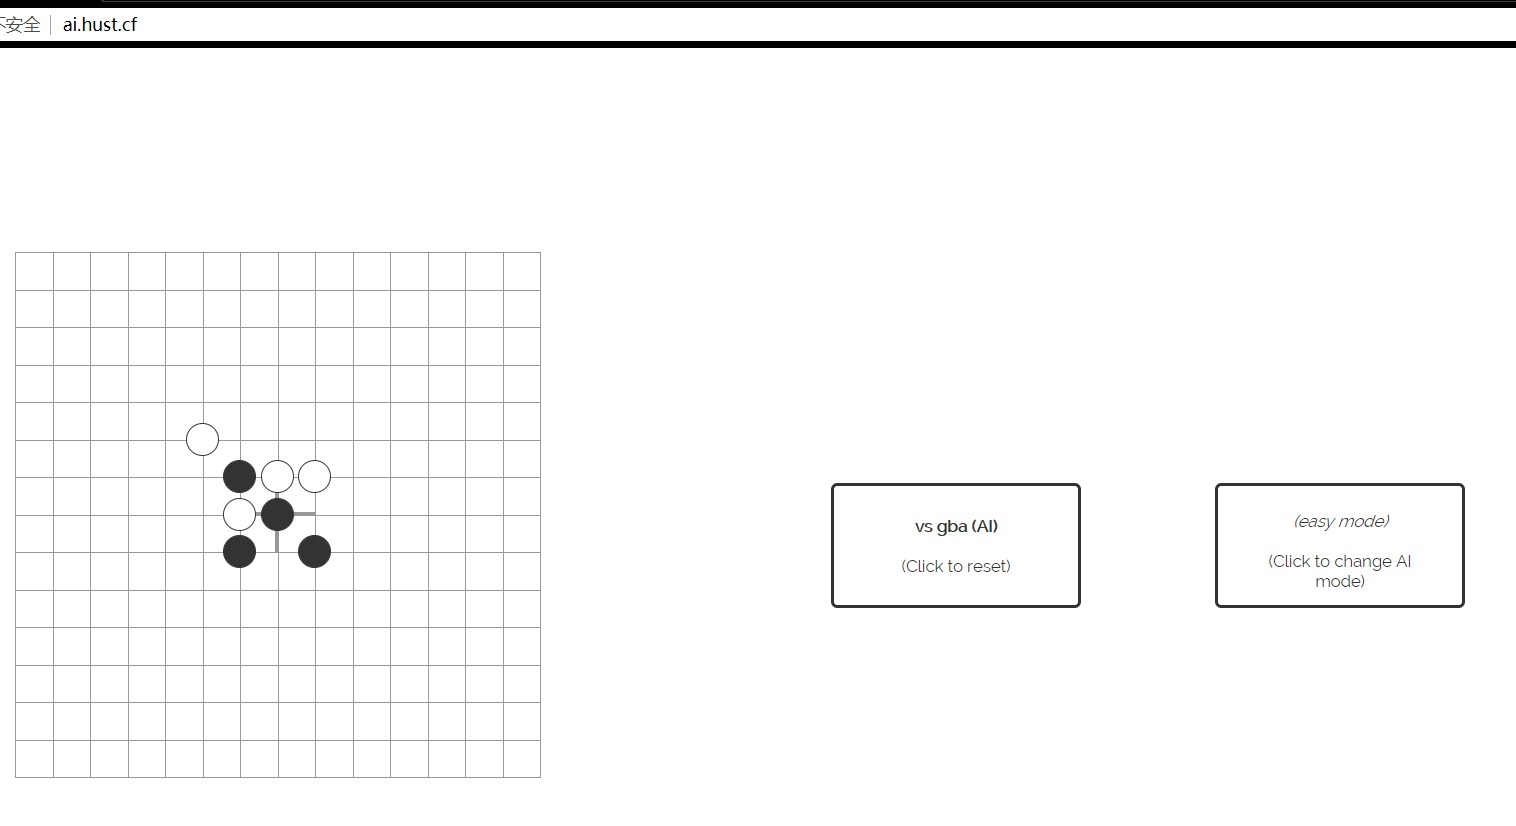
\includegraphics[width=\textwidth,height=7cm]{figures/final_UI.png}
  \caption{五子棋游戏主界面}
  \label{fig:UI}
\end{figure}

\subsection{五子棋人工智能实现}
本文的蒙特卡洛树搜索框架参考了 Michael Liu 的一篇文章\cite{web:medium_mcts},
其对于 UCT 算法的实现细节主要参考了 Sylvai Gelly 的一篇文章\cite{DBLP:journals/ai/GellyS11}。
本节主要阐述 MCTS.js 模块中的一些实现细节。
\subsubsection{智能主流程}
对于给定游戏状态(棋局分布),GBA 系统通过 2 步给出下一步理想落子。首先,通过蒙特卡洛树搜索 4 个阶段收集足够的游戏统计信息;
然后,通过分析这些游戏统计信息,给出下一步理想落子。

其基本框架如流程~\ref{alg:mcts_main}所示。
根据当前游戏状态,创建搜索树根节点。
接下来进行 4 阶段的不停迭代,直到达到时限。
首先,在当前深度选择一个 UCT 值最大的节点,若游戏未到此步结束,
则在此节点基础上扩展一个新的子节点,然后沿着此路径进行随机模拟,直至游戏结束。
最后根据游戏结果,回播游戏统计信息,完成一次 4 阶段迭代。

\begin{algorithm}
  \floatname{algorithm}{流程}
	\algrenewcommand{\algorithmicrequire}{\textbf{输入:}}
	\algrenewcommand{\algorithmicensure}{\textbf{输出:}}
	\caption{GBA 系统主流程}
	\label{alg:mcts_main}
  \begin{algorithmic}[1]
    \Function{runSearch}{$state$, $timeout$}
      \State $rootNode \gets$ makeNode($state$)
      \While{未到 $timeout$ 时限}
        \State $node \gets$ MCTS.select($state$)
        \State $winner \gets$ StateMachine.checkWinner($node.state$)
        \If{isNotLeaf($node$) AND 未决出胜者 $winner$}
          \State $node \gets nextNode \gets$ MCTS.expand($node$)
          \State $winner \gets$ MCTS.simulate($node$)
        \EndIf
        \State MCTS.backpropagate($node$, $winner$)
      \EndWhile
    \EndFunction
	\end{algorithmic}  
\end{algorithm}

\subsubsection{选择过程}
如流程~\ref{alg:mcts_select}所示,首先,根据游戏状态找到搜索树根节点;
然后,根据当前状态所有可行解,确定下一步落子集合;
在落子集合中,找出 UCT 值最大的节点便可完成选择。

\begin{algorithm}
  \floatname{algorithm}{流程}
	\algrenewcommand{\algorithmicrequire}{\textbf{输入:}}
	\algrenewcommand{\algorithmicensure}{\textbf{输出:}}
	\caption{GBA 系统选择过程}
	\label{alg:mcts_select}
  \begin{algorithmic}[1]
    \Function{select}{$state$}
      \State $node \gets$ Tree.getNode($state$)
      \While{$node$ 存在未扩展的子节点}
        \State $plays \gets$ node.allPlays($state$)
        \State $childNodes \gets$ Tree.getNodes($plays$)
        \State $bestNode \gets$ maxUCT($childNodes$)
        \State $node \gets bestNode$
      \EndWhile
      \State \textbf{return} $node$
    \EndFunction
	\end{algorithmic}  
\end{algorithm}

\subsubsection{扩展过程}
如流程~\ref{alg:mcts_expand}所示,
对于上一阶段选取的节点,计算其下一步可能进行的所有未扩展的落子,
选定一个可能的落子,计算新的游戏状态,扩展子节点,将新扩展的子节点插入搜索树。

\begin{algorithm}
  \floatname{algorithm}{流程}
	\algrenewcommand{\algorithmicrequire}{\textbf{输入:}}
	\algrenewcommand{\algorithmicensure}{\textbf{输出:}}
	\caption{GBA 系统扩展过程}
	\label{alg:mcts_expand}
  \begin{algorithmic}[1]
    \Function{expand}{$node$}
      \State $plays \gets$ unexpandedPlays($node$)
      \State $play \gets$ random($plays$)
      \State $childState \gets$ StateMachine.nextState($node.state$, $play$)
      \State $childNode \gets$ expandChild($node$)
      \State $Tree \gets$ Tree.insert($cihldNode$)
      \State \textbf{return} $childNode$
    \EndFunction
	\end{algorithmic}  
\end{algorithm}

\subsubsection{模拟过程}
如流程~\ref{alg:mcts_simulate}所示,
从上一阶段扩展的节点开始,根据其对应的游戏状态,
计算其下一步可行的落子集合,
随机选取一个落子,计算出新的游戏状态,
若决出胜者,则终止此轮模拟;
否则,根据新的游戏状态继续落子。

\begin{algorithm}
  \floatname{algorithm}{流程}
	\algrenewcommand{\algorithmicrequire}{\textbf{输入:}}
	\algrenewcommand{\algorithmicensure}{\textbf{输出:}}
	\caption{GBA 系统模拟过程}
	\label{alg:mcts_simulate}
  \begin{algorithmic}[1]
    \Function{simulate}{$node$}
      \State $state \gets$ state($node$)
      \State $winner \gets$ StateMachine.checkWinner($state$)
      \While{未决出胜者 $winner$ OR 达成和局}
        \State $plays \gets$ allLegalPlays($state$)
        \State $play \gets$ random($plays$)
        \State $state \gets$ StateMachine.nextState($state$, $play$)
        \State $winner \gets$ StateMachine.checkWinner($state$)
      \EndWhile
      \State \textbf{return} $winner$
    \EndFunction
	\end{algorithmic}  
\end{algorithm}

\subsubsection{回播过程}
如流程~\ref{alg:mcts_backpropagate}所示,
从扩展阶段得到的节点开始,向搜索树根节点开始反向遍历(父亲节点),
根据游戏结果,增加每个节点的模拟计数与胜利计数,
从而完成游戏信息回播。

\begin{algorithm}
  \floatname{algorithm}{流程}
	\algrenewcommand{\algorithmicrequire}{\textbf{输入:}}
	\algrenewcommand{\algorithmicensure}{\textbf{输出:}}
	\caption{GBA 系统回播过程}
	\label{alg:mcts_backpropagate}
  \begin{algorithmic}[1]
    \Function{backpropagate}{$node$, $winner$}
      \While{未到根节点}
        \State s($node$) $+= 1$
        \If{$node.player === $ reverse($winner$)}
          \State w($node$) $+= 1$
        \EndIf
        \State $node \gets$ parent($node$)
      \EndWhile
    \EndFunction
	\end{algorithmic}  
\end{algorithm}

\subsubsection{选出理想落子}
在规定时限($timeout$)到达后,
完成了 $N$ 轮蒙特卡洛树搜索 4 阶段迭代。
根据节点上得到的游戏统计信息,选出下一步的理想落子。
GBA 系统简单地选择胜率最高的落子,即拥有 $w_i/s_i$ 最大值的落子。

\clearpage

\section{五子棋对弈算法优化}
\subsection{计分板优化策略}
由于性能限制,如果对于所有空格位置处都进行随机搜索的话,
会使得 GBA 系统在限定的时间内(例如 3 秒) 无法得出最有效的落子选择,
使得其最后的落子选择异常糟糕,造成一种“人工智障”的戏剧场面。

利用计分板策略计算当前棋局局势,得出下一步较为优势的落子集合,缩小搜索树,
可以大幅度提升 GBA 系统的落子选择表现。

计分板优化策略根据五子棋的领域知识,对棋盘上所有可行落子的地方进行打分。
如某落子处在某一方向(横/竖/左斜/右斜)形成了“杀4”(即阻断对方五子连续)局势,
则为该处落子增加 50000 分;
如某落子处在某一方向(横/竖/左斜/右斜)形成了“活3”(即本方三子连续,且两端都有空位)局势,
则为该处落子增加 50 分;
如某落子处在某一方向(横/竖/左斜/右斜)形成了“死3”(即本方三子连续,只有一端都有空位)局势,
则为该处落子增加 25 分;
如某落子处在某一方向(横/竖/左斜/右斜)形成了“连5”(即本方五子连续)局势,
则为该处落子增加 90000 分。

采取一系列类似的策略,得到所有可行落子的评分集合,称为计分板。
选取计分板中得分较高的一些落子,放入下一步可行落子集合,
返回给 GBA 系统进行蒙特卡洛树搜索的扩展和模拟阶段。
所有计分策略与对应分数如表~\ref{tab:score_board}所示。

\begin{table}[htbp]
  \caption{计分板策略分数评定}
  \label{tab:score_board}
  \centering
  \begin{tabular}[c]{l|l}
    \hline
    \multicolumn{1}{c|}{\textbf{局势}} & 
    \multicolumn{1}{c}{\textbf{分数}} \\
    \hline
	  杀 2 & 10 \\
	  杀 3(一端空位)& 30 \\
	  杀 3 (两端空位)& 40 \\
	  杀 4(一端空位)& 60 \\
	  杀 4 (两端空位)& 110 \\
	  杀 5 & 50100 \\
	  活 2 & 10 \\
	  死 3 & 25 \\
	  活 3 & 50 \\
	  死 4 & 55 \\
	  活 4 & 100 \\
	  活 5 & 90000 \\
   \hline
  \end{tabular}
\end{table}

\subsection{算法优化结果}
当玩家执黑子(先手),GBA 系统执白子时,在采取随机模拟策略时,其落子表现如图~\ref{fig:mcts_gba_v1}所示。
在利用计分板策略对对弈策略进行优化后,其落子表现如图~\ref{fig:mcts_gba_v2}所示。可以看到,其落子表现得到了极大提升。

\begin{figure}[htb]
  \centering
  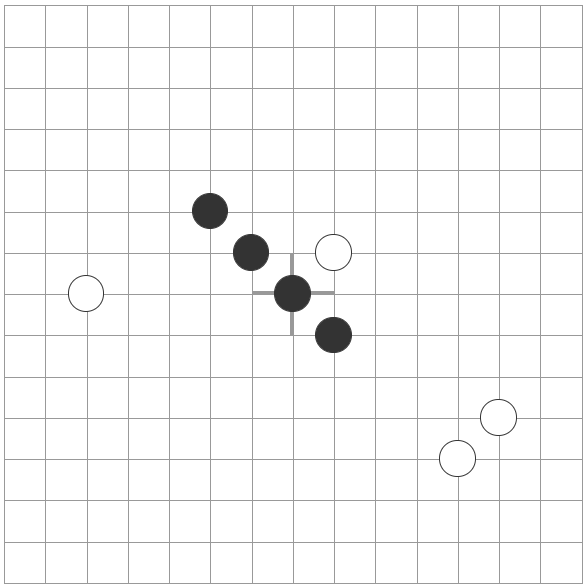
\includegraphics[width=0.5\textwidth,height=5cm]{figures/final_gba_v1.png}
  \caption{GBA 系统落子表现(随机模拟策略)}
  \label{fig:mcts_gba_v1}
\end{figure}

\begin{figure}[htb]
  \centering
  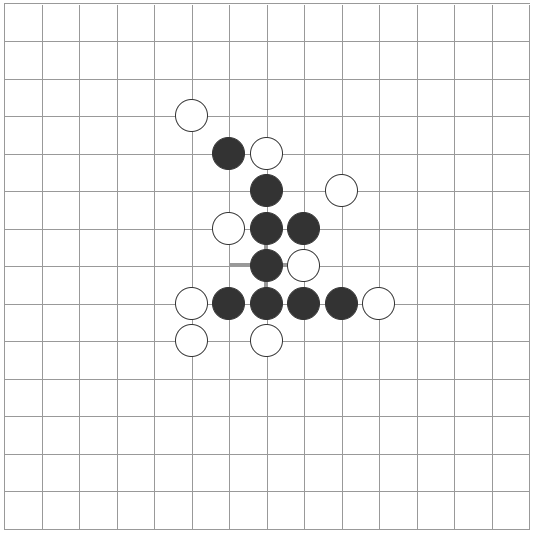
\includegraphics[width=0.5\textwidth,height=5cm]{figures/final_gba_v2.png}
  \caption{GBA 系统落子表现(计分板策略优化)}
  \label{fig:mcts_gba_v2}
\end{figure}

\clearpage

\section{总结}
GBA 系统实现了基本的对弈功能,但受限于浏览器的运算能力,
其棋力还十分地孱弱。在使用随机模拟策略时,其落子选择表现异常糟糕。
利用计分板策略进行优化后,才使得其消除了极为糟糕的落子选择(如未能杀 4)。
希望未来能有机会将其蒙特卡洛树搜索部分移植到系统语言上,
JavaScript 只实现图形界面部分,从而提升 GBA 系统的棋力。
本系统代码尚未开源,若需获取源代码,请通过邮箱联系本文作者(~\href{mailto:sabertazimi@gmail.com}{sabertazimi@gmail.com})。
\newpage

\bibliographystyle{unsrt}
\bibliography{bibs/report}
\addcontentsline{toc}{section}{\S 参考文献}
\newpage

\end{document}
